\begin{figure*}[t]
  \centering
  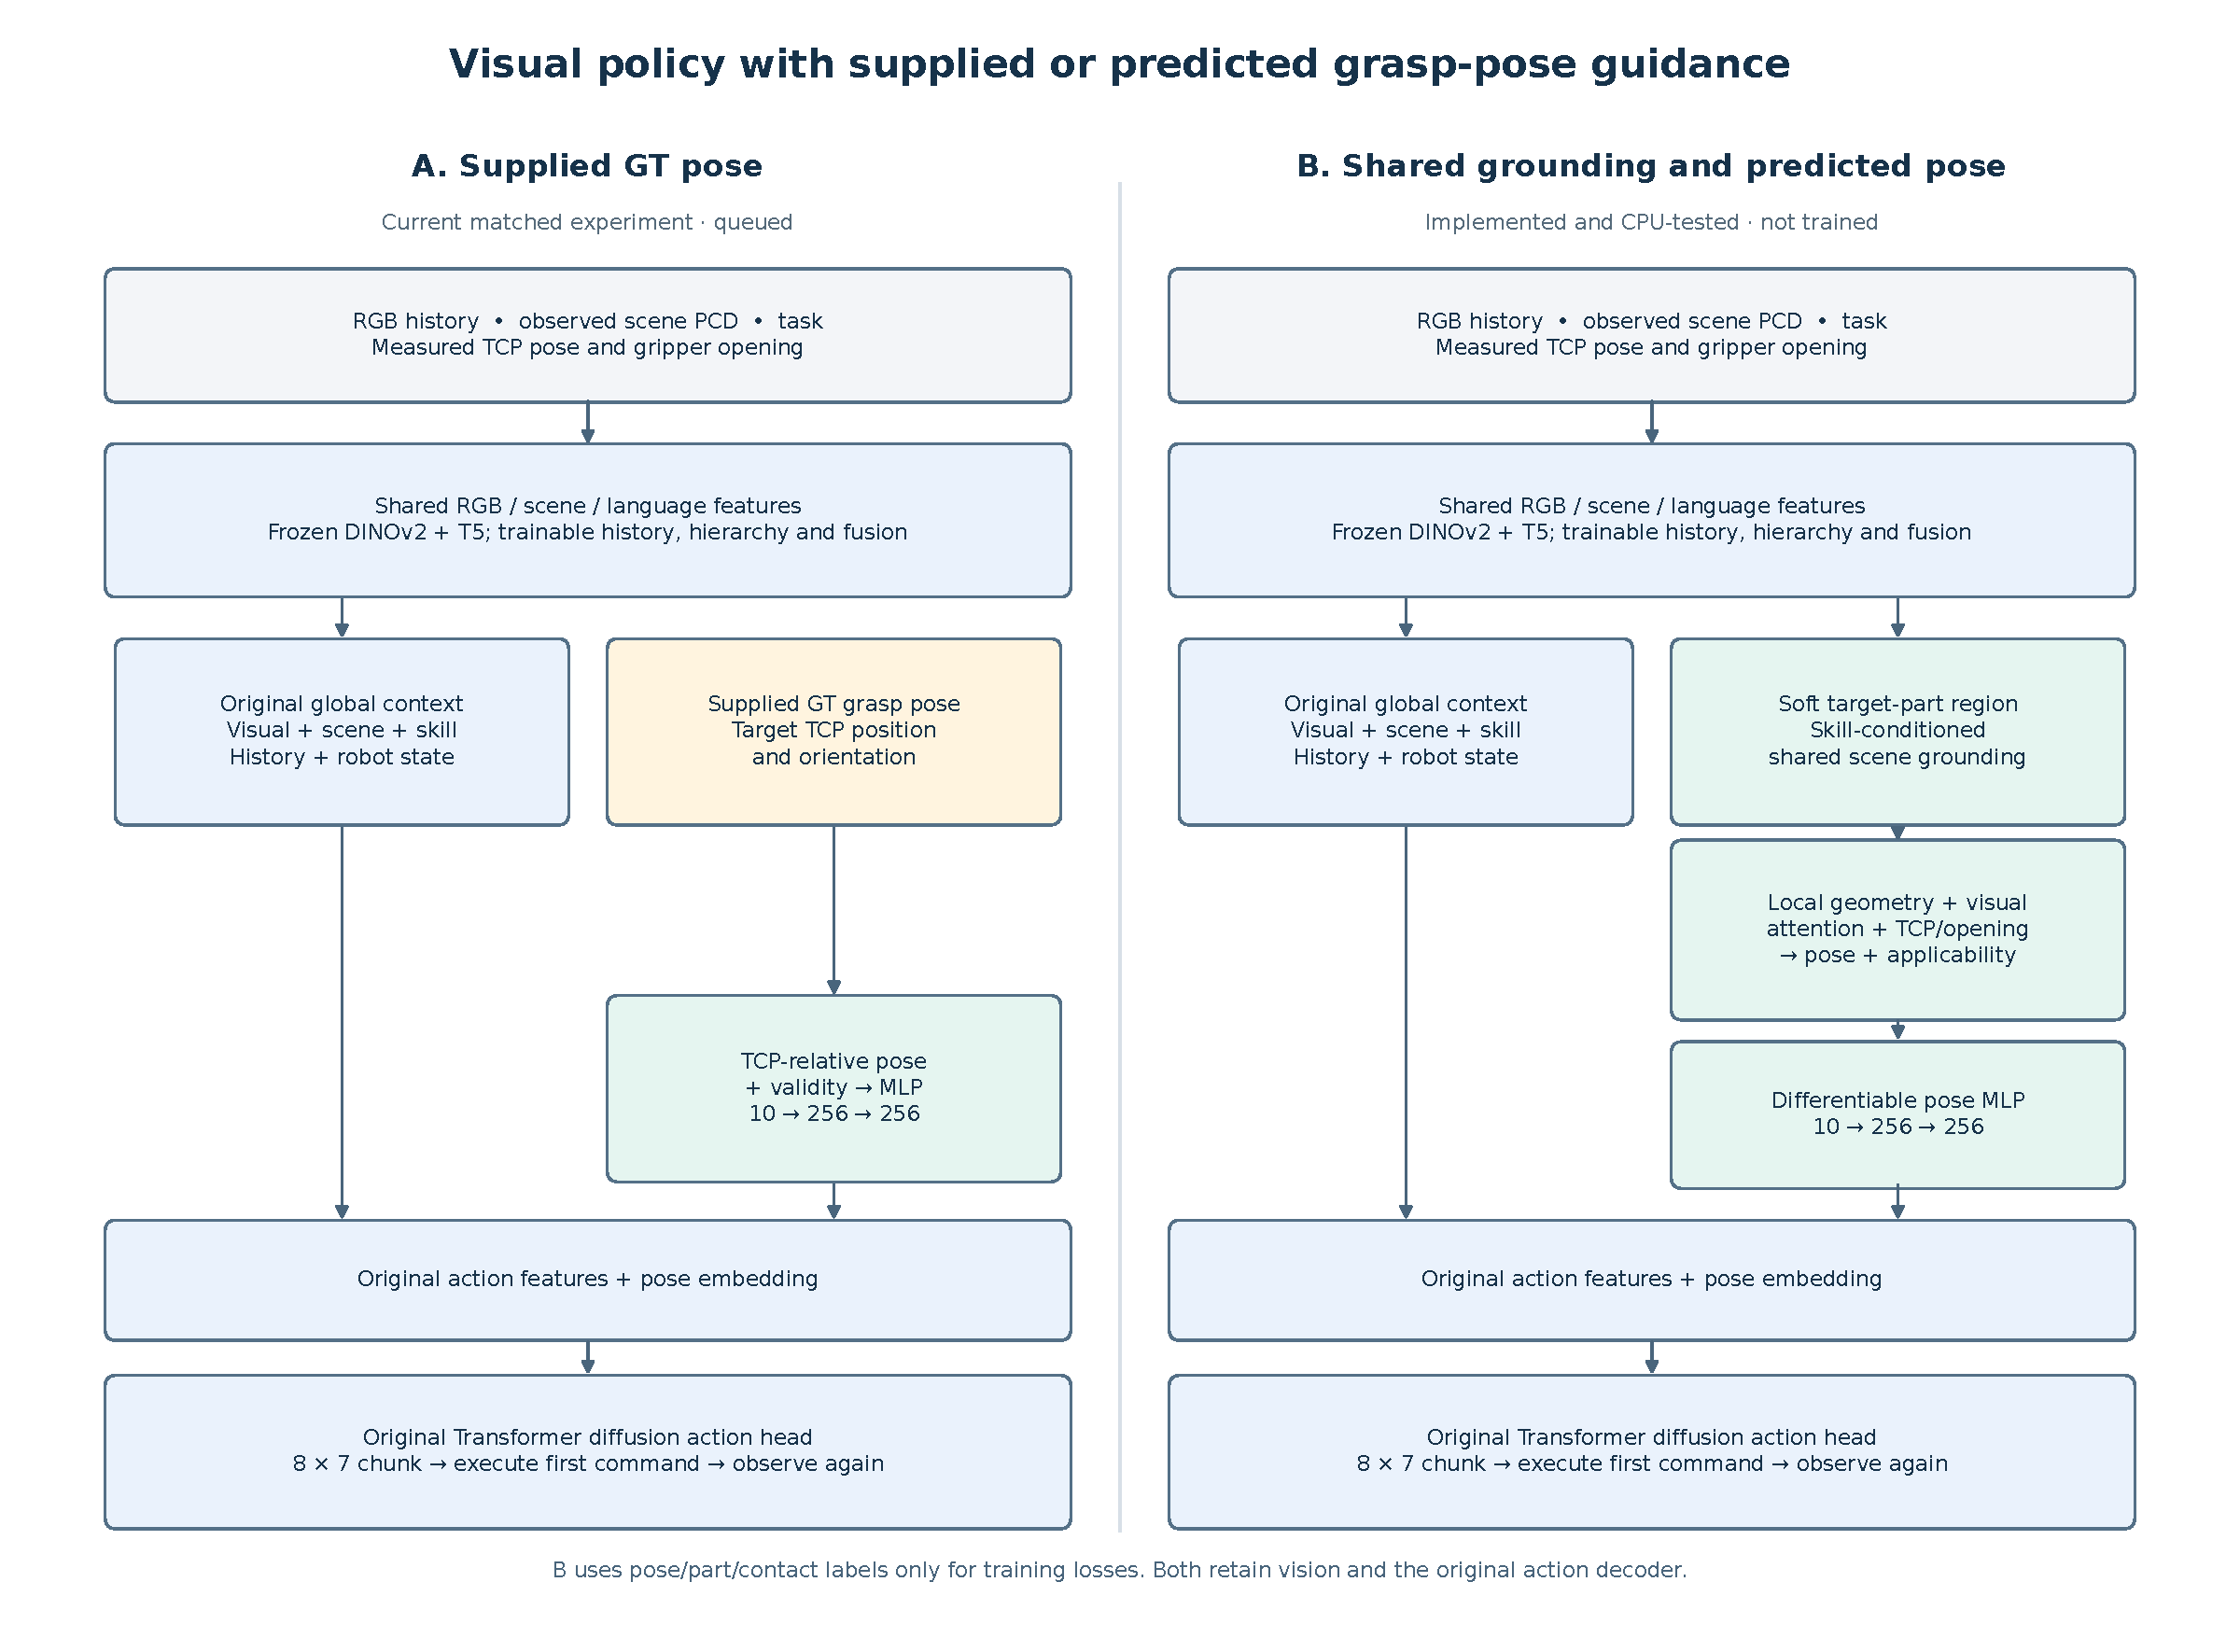
\includegraphics[width=\textwidth]{visual_pose_architectures.pdf}
  \caption{Two visual-policy pose-conditioning paths. (A) The current matched
  experiment supplies an oracle first-grasp TCP pose. (B) The implemented next
  architecture predicts a target TCP pose from shared skill-conditioned scene
  grounding, local geometry, visual attention and measured robot state. Its
  differentiable pose embedding conditions the original diffusion action head
  alongside the global visual context. Part/contact and pose labels supervise
  training only in B. DINO/T5 remain frozen; shared policy layers fine-tune and
  new pose layers learn jointly. B has not yet been trained or evaluated.}
  \label{fig:visual-pose-architectures}
\end{figure*}
